\documentclass[tikz, 12pt, a4paper]{report}
\usepackage[T1]{fontenc}
\usepackage{caption}
\usepackage{subcaption}
\usepackage[usenames, dvipsnames, rgb]{xcolor}
\usepackage{tikz}
\usepackage{pgf-pie}
\usetikzlibrary{arrows, positioning, shadows}
\begin{document}
\begin{figure}[!htbp]
\centering
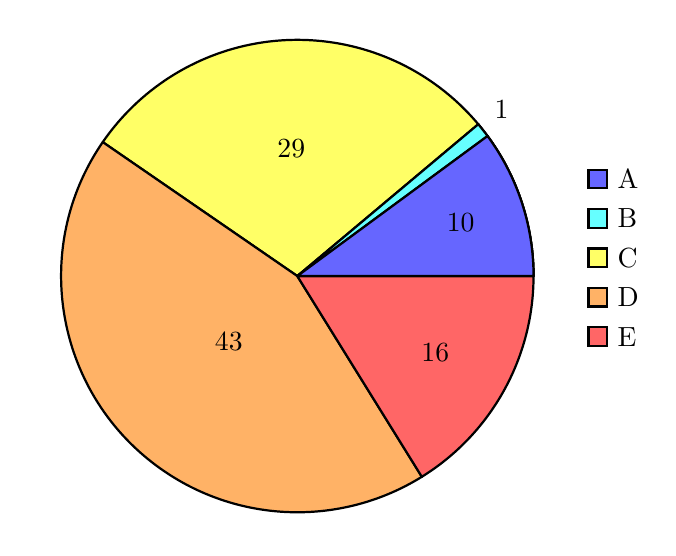
\begin{tikzpicture}
\pie[sum=auto,text=legend]{10/A, 1/B, 29/C, 43/D, 16/E}
% COMMENT EDIT: 10+1+29+43+16 = 99 !!!
\pie[sum=99, hide number]{10/, 1/1}
\pie[sum=99]{10/}
\end{tikzpicture}
\caption{Pie}
\end{figure}
\end{document}
